\documentclass[aspectratio=169,11pt]{beamer}

% Shared style (ib-tutorials.sty at the repo root).
\makeatletter\def\input@path{{./}{../}}\makeatother
\usepackage{ib-tutorials}

\usepackage[utf8]{inputenc}
\usepackage{amsmath,amssymb}
\usepackage{booktabs}
\usepackage{array}
\newcolumntype{L}[1]{>{\raggedright\arraybackslash}p{#1}}
\usepackage{graphicx}
\graphicspath{{../pictures/3-ibamr-fundamentals/}{pictures/3-ibamr-fundamentals/}}
\usepackage{xcolor}
\usepackage{listings}
\usepackage{tikz}
\usetikzlibrary{arrows.meta,positioning,shapes.geometric,fit,calc,decorations.pathmorphing}
\usepackage{hyperref}

\newcommand{\sourcecredit}[1]{\vfill\begin{flushright}\tiny\textcolor{DarkGray}{#1}\end{flushright}}

\lstset{
  basicstyle=\ttfamily\scriptsize\color{BlackGray},
  keywordstyle=\color{NavyBlue}\bfseries,
  commentstyle=\color{DarkGray}\itshape,
  stringstyle=\color{OliveGreen},
  showstringspaces=false,
  columns=fullflexible,
  keepspaces=true,
  breaklines=true,
  breakindent=1em,
  frame=single,
  framerule=0.4pt,
  rulecolor=\color{LightGray},
  backgroundcolor=\color{LightGray!30},
  xleftmargin=0.25em,
  xrightmargin=0.25em
}
\lstdefinestyle{shell}{morecomment=[l]{\#}}
\lstdefinestyle{input}{morecomment=[l]{//}}
\lstdefinestyle{matlab}{morecomment=[l]{\%}}
\lstdefinestyle{python}{morecomment=[l]{\#}}
\lstdefinestyle{data}{}
\lstdefinestyle{tiny}{basicstyle=\ttfamily\tiny\color{BlackGray}}
\lstdefinestyle{inputtiny}{morecomment=[l]{//},basicstyle=\ttfamily\tiny\color{BlackGray}}
\lstdefinestyle{matlabtiny}{morecomment=[l]{\%},basicstyle=\ttfamily\tiny\color{BlackGray}}
\lstdefinestyle{cpp}{language=C++,morecomment=[l]{//}}
\lstdefinestyle{cpptiny}{language=C++,morecomment=[l]{//},basicstyle=\ttfamily\tiny\color{BlackGray}}
\lstdefinestyle{cmake}{morecomment=[l]{\#}}

\title[Custom spring forces and active pumping]{Custom spring forces and active pumping}
\subtitle{Writing your own spring force function, applying forces to a structure, and driving a heart tube three ways}
\author[Miller]{Laura A. Miller}
\institute[UArizona]{Department of Mathematics, University of Arizona}
\date{Using IB Software \textbullet\ Part III \textbullet\ Chapter 9b}

\begin{document}

% 1
\begin{frame}[plain]
\maketutorialtitlepanel{%
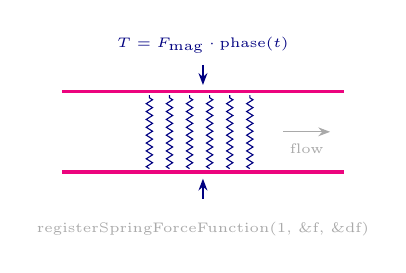
\begin{tikzpicture}[scale=0.85]
  \draw[RubineRed,very thick] (0,1.6) -- (4.2,1.6);
  \draw[RubineRed,very thick] (0,0.4) -- (4.2,0.4);
  \foreach \x in {1.3,1.6,...,2.9}{\draw[decorate,decoration={zigzag,segment length=1mm,amplitude=0.4mm},NavyBlue] (\x,0.45) -- (\x,1.55);}
  \draw[NavyBlue,thick,-{Stealth[length=1.5mm]}] (2.1,2.0) -- (2.1,1.7);
  \draw[NavyBlue,thick,-{Stealth[length=1.5mm]}] (2.1,0.0) -- (2.1,0.3);
  \node[font=\tiny,text=NavyBlue] at (2.1,2.3) {$T = F_{\mathrm{mag}}\cdot\mathrm{phase}(t)$};
  \draw[-{Stealth[length=1.5mm]},DarkGray] (3.3,1.0) -- (4.0,1.0);
  \node[font=\tiny,text=DarkGray] at (3.65,0.75) {flow};
  \node[font=\tiny,text=DarkGray] at (2.1,-0.45) {\code{registerSpringForceFunction(1, \&f, \&df)}};
\end{tikzpicture}}
\end{frame}

% 2
\begin{frame}{Learning goals}
\label{fr:goals}
\footnotesize By the end of this chapter you should be able to:
\begin{enumerate}
  \item write a spring force function of your own (a nonlinear spring, a muscle, an applied force), register it with IBAMR's force generator under a force-function index, and select it per spring from the \code{.spring} file;
  \item use the spring's parameters for whatever your law needs, and change them in time from an update function, since the force function itself never sees the time;
  \item drive a structure with an applied force rather than with target points, and say when each is the better choice;
  \item read and run the heart-tube pump example (IB/11) in its five actuation modes: suction pumping by target points or by force, peristalsis by a travelling force, a travelling stiffness, or travelling targets;
  \item know the other ways to put a force on a structure (a Lagrangian force strategy, a uniform body force, an Eulerian forcing function) and recognize the mistakes that make an applied force do nothing or too much.
\end{enumerate}
\begin{punchbox}
\footnotesize Chapter 9a moved target points and changed springs; this chapter changes the law of the spring. Chapter 36 (Part VI) builds the two-point valveless pump on the same ideas; chapter 11 reads the forces out.
\end{punchbox}
\end{frame}

% 3
\begin{frame}{How this chapter was checked}
\label{fr:checked}
\begin{itemize}\footnotesize
  \item The force-function interface is quoted from the IBAMR 0.19.0 headers (\code{IBSpringForceFunctions.h}, \code{IBStandardForceGen.h}) and from the force generator's source; the 2013 interface the course first taught is shown next to it (slide \ref{fr:old}).
  \item The example IB/11 (heart-tube pump) is the lab's 2014 \code{Forced-tube-pump} code ported to IBAMR 0.16.0 and 0.19.0, with the five actuation modes of the 2014 lecture and code selectable from the input file; it builds with 0 warnings, four modes run two periods with the shipped settings, and the fifth (the stiffness wave) stops at $0.64$ s when the walls stick, which is reported as such (slides \ref{fr:wrong2}, \ref{fr:fmag}). The figures are from those runs.
  \item The 2014 lecture's code had an undefined variable, a loop that added packets that had left the tube, a rest-length slot reused as a phase, and a structure-order dependency; each is named on the slide where it occurs and fixed in IB/11. Its three peristalsis modes, run as written, aborted before $0.8$ s; the slide ``What can go wrong (2)'' shows why, and the shipped parameters were chosen from runs that complete.
  \item The Python generator writes files identical to the MATLAB one (Octave 8.4 against Python 3.12, 27 files, token for token).
\end{itemize}
\begin{punchbox}
\footnotesize Slide numbers refer to this deck; chapter numbers (3, 5, 6, 7, 8a, 8b, 9a, 11, 15, 26, 36) to the other chapters of this series.
\end{punchbox}
\end{frame}

% 4
\begin{frame}{Where to look things up}
\label{fr:lookup}
\small
\begin{itemize}
  \item \al{The interface}: \code{include/ibamr/IBSpringForceFunctions.h} defines the two function-pointer types and the default Hookean law, with its documentation; \code{IBStandardForceGen.h} declares \code{registerSpringForceFunction}. The 2013 slides called the first file \code{IBSpringFunction.h}, which never existed under that name.
  \item \al{The upstream example}: \code{examples/IB/explicit/ex3} registers its own linear spring law (slide \ref{fr:ex3}); the 2013 and 2014 lectures both pointed to it.
  \item \al{The force generator}: \code{src/IB/IBStandardForceGen.cpp}, the loop of chapter 8b that calls your function once per spring per force evaluation.
  \item \al{The examples of this series}: IB/11 (this chapter), with its \code{main.cpp} (the force functions and their registration), five update functions, five input files and a README with the measured results; IB/06 (chapter 9a) for the update-function pattern.
  \item The IBAMR FAQ, \url{https://github.com/IBAMR/IBAMR/wiki/FAQ}, and the class documentation, \url{https://ibamr.github.io/docs}.
\end{itemize}
\end{frame}

% 5
\begin{frame}{Why new spring functions?}
\label{fr:why}
\small From the October 2013 lecture, \emph{Creating your own spring function in IBAMR}:
\begin{itemize}
  \item ``If you want a nonlinear spring or a spring that behaves like a muscle, you may need to create a new spring function.''
  \item ``IBAMR has a way to do this by registering your function and giving your type of spring a number that can be used in \code{.spring} files.''
  \item ``Set up a spring function and register it with the \code{IBStandardForceGen} object that is created in the main routine. If you use function index 0 when registering your spring function, your function will become the `default' spring function.''
  \item ``Note that you can set the spring function number in the \code{.spring} file. E.g.\ different spring functions can be assigned to different links.''
\end{itemize}
\vspace{1mm}
\begin{punchbox}
\small A ``spring'' in IBAMR is any force between two points that acts along the line joining them and depends on their distance and on numbers you store with the spring. Hooke's law is the default; a muscle, a cable that goes slack, a nonlinear tissue law, or a force you apply from outside (this chapter's pump) are all springs with a different function. ``The force will be applied along the (normalized) fiber connecting the two node points'' (2015).
\end{punchbox}
\end{frame}

% 6
\begin{frame}[fragile]{The interface, in IBAMR 0.19.0}
\label{fr:interface}
\begin{columns}[T,onlytextwidth]
\begin{column}{0.58\textwidth}
\begin{lstlisting}[style=cpptiny]
// include/ibamr/IBSpringForceFunctions.h (0.19.0)
// A spring force function returns the (undirected) "tension" T from
//   R              the distance between the "master" and "slave" nodes
//   params         the numbers on the spring's line of the .spring file
//   lag_mastr_idx  the Lagrangian index of the master node
//   lag_slave_idx  the Lagrangian index of the slave node
using SpringForceFcnPtr =
    double (*)(double R, const double* params, int lag_mastr_idx, int lag_slave_idx);
// The derivative dT/dR, same arguments
using SpringForceDerivFcnPtr =
    double (*)(double R, const double* params, int lag_mastr_idx, int lag_slave_idx);

// The default, force function index 0: a Hookean spring
inline double default_spring_force(double R, const double* params, int, int)
{
    return params[0] * (R - params[1]);   // stiffness * (length - rest length)
}
inline double default_spring_force_deriv(double, const double* params, int, int)
{
    return params[0];
}
\end{lstlisting}
\end{column}
\begin{column}{0.4\textwidth}
\footnotesize Your function returns one number, the \al{tension} $T$: positive pulls the two points together, negative pushes them apart. The generator turns it into the two forces (chapter 8b's listing):
\begin{gather*}
  \mathbf{F}_{\mathrm{master}} = T\,\frac{\mathbf{X}_{\mathrm{slave}} - \mathbf{X}_{\mathrm{master}}}{R},\\
  \mathbf{F}_{\mathrm{slave}} = -\mathbf{F}_{\mathrm{master}}.
\end{gather*}
\footnotesize If $R$ is below machine precision the generator skips the spring, so your function never divides by zero. The default is Hooke's law with the stiffness in \code{params[0]} and the rest length in \code{params[1]}; chapter 6 explains why the file stiffness is $K/\Delta s$.
\end{column}
\end{columns}
\end{frame}

% 6b
\begin{frame}[fragile]{The interface (2): parameters, indices, derivative}
\label{fr:interface2}
\begin{lstlisting}[style=cpptiny]
// include/ibamr/IBStandardForceGen.h: give the function a number
void registerSpringForceFunction(int force_fcn_index,
                                 const SpringForceFcnPtr spring_force_fcn_ptr,
                                 const SpringForceDerivFcnPtr spring_force_deriv_fcn_ptr = nullptr);
\end{lstlisting}
\begin{itemize}\footnotesize
  \item \code{params} is the spring's own line of the file after the two indices: as many numbers as you wrote, in that order (chapter 9a); the default reads two. They are stored per spring, so two springs with the same index can carry different numbers.
  \item The two indices let a law depend on \emph{which} spring it is (a stiffness that varies along a fibre, a different rest length at the ends) without extra parameters.
  \item The derivative $dT/dR$ is used only when IBAMR needs the Jacobian of the forces (implicit time stepping, chapter 15). Pass \code{nullptr} and the generator estimates it by a centred finite difference with step $\max(R,1)\,\epsilon^{1/3}$; pass the true derivative and it is exact and cheap.
  \item The force function index is an \code{int} of your choosing; the constructor of \code{IBStandardForceGen} registers the default under 0 before you get the object.
\end{itemize}
\end{frame}

% 7
\begin{frame}[fragile]{The 2013 interface, for reading old code}
\label{fr:old}
\vspace{-1mm}
\begin{columns}[T,onlytextwidth]
\begin{column}{0.52\textwidth}
\footnotesize The 2013 lecture showed the then-current default from \code{IBSpringForceFunctions.h}:
\begin{lstlisting}[style=cpptiny]
inline void
default_linear_spring_force(double F[NDIM], const double D[NDIM],
    const double& stf, const double& rst,
    const int& lag_mastr_idx, const int& lag_slave_idx)
{
    // Compute the distance between the "master" and "slave" nodes.
    double R_sq = 0.0;
    for (int d = 0; d < NDIM; ++d) R_sq += D[d]*D[d];
    const double R = sqrt(R_sq);
    // Compute the force applied to the "master" node.
    const double& kappa = stf;
    const double& R0 = rst;
    if (R > std::numeric_limits<double>::epsilon())
        for (int d = 0; d < NDIM; ++d)
            F[d] = kappa*(1.0-(R0/R))*D[d];
    else
        for (int d = 0; d < NDIM; ++d) F[d] = kappa*D[d];
    return;
}
// and in the constructor (2013), then as now:
IBStandardForceGen::IBStandardForceGen()
{ registerSpringForceFunction(0, &default_spring_force, &default_spring_force_deriv); }
\end{lstlisting}
\end{column}
\begin{column}{0.46\textwidth}
\scriptsize
\setlength{\tabcolsep}{3pt}
\begin{tabular}{@{}L{0.2\textwidth}L{0.36\textwidth}L{0.38\textwidth}@{}}
\toprule
 & 2013 & 2015 onward, 0.19.0\\
\midrule
returns & nothing; fills \code{F[NDIM]}, the force vector on the master & \code{double}, the tension $T$; the generator makes the vectors\\
distance & \code{D[NDIM]}, the displacement vector; the function computes $R$ & \code{R}, already computed\\
parameters & two named arguments, \code{stf} and \code{rst} & \code{const double* params}, any number of them\\
derivative & none & a second function, or \code{nullptr}\\
header name in the slides & \code{IBSpring\allowbreak Function.h} & \code{IBSpringForce\allowbreak Functions.h}\\
\bottomrule
\end{tabular}

\scriptsize Porting a 2013 function: compute $T$ from $R$ and \code{params} (for the law above, $T = \kappa(R - R_0)$, which is \code{kappa*(1 - R0/R)*R}), drop the loops, and add a derivative. The zero-distance guard is now inside the generator.
\end{column}
\end{columns}
\end{frame}

% 8
\begin{frame}[fragile]{The upstream example: ex3 overrides the default}
\label{fr:ex3}
\begin{columns}[T,onlytextwidth]
\begin{column}{0.52\textwidth}
\begin{lstlisting}[style=cpptiny]
// examples/IB/explicit/ex3/example.cpp (0.19.0): a linear spring written in strain
inline double
linear_spring_force(double R, const double* params, int /*lag_mastr_idx*/, int /*lag_slave_idx*/)
{
    const double stf = params[0];
    const double rst = params[1];
    return stf * (R / rst - 1.0);
}
inline double
linear_spring_force_deriv(double /*R*/, const double* params, int /*lag_mastr_idx*/, int /*lag_slave_idx*/)
{
    const double stf = params[0];
    const double rst = params[1];
    return stf / rst;
}
...
Pointer<IBStandardForceGen> ib_force_fcn = new IBStandardForceGen();
ib_force_fcn->registerSpringForceFunction(0, &linear_spring_force, &linear_spring_force_deriv);
ib_method_ops->registerIBLagrangianForceFunction(ib_force_fcn);
\end{lstlisting}
\end{column}
\begin{column}{0.46\textwidth}
\scriptsize ``Note that the first argument to \code{registerSpringForceFunction()} is the force function index. In the example, the default linear spring function (force function index 0) is overridden. If you wanted to make a different function that can be used with the default, assign your new function some other integer index.'' (2013, 2014)
\begin{itemize}
  \item ex3's law is Hooke's law written in \al{strain}: $T = \kappa\,(R/r_0 - 1) = (\kappa/r_0)(R - r_0)$. The same spring as the default, but its file stiffness means force per unit \emph{strain}, which is chapter 6's $K$, not $K/\Delta s$: overriding index 0 changes what every number in every \code{.spring} file means. Say so in the generator when you do it.
  \item The derivative is given exactly, $\kappa/r_0$.
  \item ex3 is the filament of chapter 13 (penalty IB, with mass); its force law is independent of that.
\end{itemize}
\end{column}
\end{columns}
\end{frame}

% 9
\begin{frame}[fragile]{The fifth column of the \code{.spring} file}
\label{fr:column}
\begin{columns}[T,onlytextwidth]
\begin{column}{0.5\textwidth}
\footnotesize ``By default, springs in \code{.spring} files get force function index 0. The \code{.spring} file format is \code{i j spring\_constant rest\_length force\_fcn\_idx}, in which $(i, j)$ is the pair of points connected by a given spring. You can mix-and-match different force function indices in the same \code{.spring} file.'' (2013, 2014)
\begin{lstlisting}[style=data]
41
0 41 5.0000000000000000e-01 0.0000000000000000e+00 1
1 42 5.0000000000000000e-01 0.0000000000000000e+00 1
...
\end{lstlisting}
\footnotesize IB/11's \code{vp\_aforce\_512.spring}: point $i$ on the top wall to point $i + 41$ below it, two parameters (here a force magnitude, $F_{\mathrm{mag}} = 0.25$, and a phase, not a stiffness and a rest length), force function 1.
\end{column}
\begin{column}{0.48\textwidth}
\footnotesize In 0.19.0 (\code{IBStandardInitializer.cpp}):
\begin{itemize}
  \item the index is read if present and \al{defaults to 0}; a line with only four numbers is a default spring;
  \item \code{uniform\_spring\_force\_fcn\_idx} in the structure's input block gives every spring of that structure the same index, like the other \code{uniform\_*} keys of chapter 6;
  \item the parameters are stored per spring as a vector; the force function receives a pointer to that spring's vector, so a line may carry three or five numbers if your law reads them (all lines of one structure should carry the same count);
  \item an index that was never registered has no function behind it: slide \ref{fr:wrong} shows what happens.
\end{itemize}
\footnotesize The generator writes the index with the line (\code{'\%d \%d \%1.16e \%1.16e \%d\textbackslash n'}); chapter 6's format table has the column.
\end{column}
\end{columns}
\end{frame}

% 10
\begin{frame}[fragile]{Writing your own: the recipe}
\label{fr:recipe}
\footnotesize Four steps, from the 2015 lecture \emph{Creating spring force functions} (Alex Hoover) and the 2014 one:
\begin{enumerate}
  \item \al{Declare the function} ``in \code{main.C}, in the function prototypes section before or after the main call'', with the interface of slide \ref{fr:interface}: \code{inline double my\_force(double R, const double* params, int lag\_mastr\_idx, int lag\_slave\_idx)}. Here ``\code{R} is the distance, \code{params} holds the two parameters (usually the spring constant and the resting length, but this can be changed)''.
  \item \al{Decide what the parameters mean} and write them into the \code{.spring} file in the generator, with the index in the fifth column.
  \item \al{Register} it ``in the `Configure the IB solver' section'':
\begin{lstlisting}[style=cpptiny]
Pointer<IBStandardForceGen> ib_force_fcn = new IBStandardForceGen();
ib_force_fcn->registerSpringForceFunction(1, &my_force, &my_force_deriv);   // the new line
ib_method_ops->registerIBLagrangianForceFunction(ib_force_fcn);
\end{lstlisting}
  \item If the law changes in time, \al{write an update function} (chapter 9a) that sets a parameter each step; the force function reads it.
\end{enumerate}
\begin{punchbox}
\footnotesize \al{The force function has no clock.} Its arguments are $R$, the parameters and the two indices; the time is not among them. Anything time-dependent must be put into a parameter by an update function before the step (the ``phase'' of the next slides), or read from a global that \code{main.cpp} sets, which is uglier. This is the single most common surprise in writing one.
\end{punchbox}
\end{frame}

% 11
\begin{frame}[fragile]{A sinusoidal force (2015)}
\label{fr:sinus}
\begin{columns}[T,onlytextwidth]
\begin{column}{0.52\textwidth}
\footnotesize ``Using this structure, let's create a simple sinusoidal force, $F = F_{\mathrm{mag}}\sin(ft)$. The force magnitude $F_{\mathrm{mag}}$ is stored in \code{params[0]}. The value of $\sin(ft)$ is stored in \code{params[1]} and will be updated in the \code{update\_springs.C} routine.''
\begin{lstlisting}[style=cpptiny]
// main.C (2015), the force function
inline double frequency_spring_force(double R, const double* params, int lag_mastr_idx, int lag_slave_idx)
{
    const double F = params[0];
    const double phase_fun = params[1];
    return F*phase_fun;
}
\end{lstlisting}
\begin{lstlisting}[style=cpptiny]
// update_springs.C (2015), "the important lines"
double freq = 1;
double theta = freq*current_time*2*pi;
const int lag_idx = node_idx->getLagrangianIndex();
double& phase = spring_spec->getParameters()[0][1];
if (muscle_lag_idxs.first <= lag_idx && lag_idx < muscle_lag_idxs.second)
{
    phase = sin(theta);
}
\end{lstlisting}
\end{column}
\begin{column}{0.46\textwidth}
\scriptsize Read together:
\begin{itemize}
  \item the \al{update function} runs before each step and writes $\sin(2\pi f t)$ into the second parameter of every spring of the ``muscle'' structure (through a reference, correctly: \code{double\& phase});
  \item the \al{force function} runs inside the step, as often as the forces are evaluated, and returns $F_{\mathrm{mag}}$ times whatever is in that slot: a tension that oscillates between $\pm F_{\mathrm{mag}}$, pulling the two points together and pushing them apart in turn, whatever their distance;
  \item the rest-length slot is \al{reused} as the phase. Nothing in IBAMR objects; only your own reading of the file must remember it.
\end{itemize}
\scriptsize The 2015 public-folder copy of this example (\code{14-YourOwnForceEx}) shipped \code{main.C} and \code{update\_springs\_freq.C} (frequency $0.86$ Hz) but no input or structure files; IB/11's \code{FORCE\_VP} mode is this force on a real structure.
\end{column}
\end{columns}
\end{frame}

% 12
\begin{frame}[fragile]{Registering it, and the derivative}
\label{fr:register}
\begin{columns}[T,onlytextwidth]
\begin{column}{0.52\textwidth}
\begin{lstlisting}[style=cpptiny]
// main.C (2015), "Configure the IB solver"; "new addition highlighted in red"
Pointer<IBStandardInitializer> ib_initializer = new IBStandardInitializer(
    "IBStandardInitializer", app_initializer->getComponentDatabase("IBStandardInitializer"));
ib_method_ops->registerLInitStrategy(ib_initializer);
Pointer<IBStandardForceGen> ib_force_fcn = new IBStandardForceGen();
ib_force_fcn->registerSpringForceFunction(1, &frequency_spring_force, &frequency_spring_force_deriv);  // <- the new line
ib_method_ops->registerIBLagrangianForceFunction(ib_force_fcn);
\end{lstlisting}
\begin{lstlisting}[style=cpptiny]
// the derivative the 2014 and 2015 lectures wrote
inline double frequency_spring_force_deriv(double R, const double* params, int lag_mastr_idx, int lag_slave_idx)
{
    return 0;
}
\end{lstlisting}
\footnotesize The public-folder slides said ``new addition highlighted in red''; the highlighting did not survive the export. The new line is the one with \code{registerSpringForceFunction(1, ...)}: index 1, so the default spring (index 0) stays available for the structure's own springs.
\end{column}
\begin{column}{0.46\textwidth}
\footnotesize About that derivative:
\begin{itemize}
  \item it is \al{correct}: $T = F_{\mathrm{mag}}\cdot\mathrm{phase}$ does not depend on $R$, so $dT/dR = 0$. The lectures did not say why it is zero, and a reader might copy it for a law that does depend on $R$, where it would be wrong;
  \item for an explicit run (all the examples here) the derivative is never called; for an implicit one it enters the Jacobian, and a wrong derivative slows or breaks the Newton solve without changing the physics;
  \item when in doubt, pass \code{nullptr}: IBAMR then differentiates $T$ numerically (\code{IBStandardForceGen.cpp}: a centred difference with a step of $\max(R, 1)\,\epsilon^{1/3}$).
\end{itemize}
\footnotesize IB/11 registers one function, \code{applied\_force}, under both indices 1 and 2 with the zero derivative; the two \code{.spring} files use one index each.
\end{column}
\end{columns}
\end{frame}

% 13
\begin{frame}{The heart-tube pump (IB/11): what it is}
\label{fr:pump}
\begin{columns}[T,onlytextwidth]
\begin{column}{0.5\textwidth}
\scriptsize The 2014 lecture \emph{Designing your own spring force function: examples for peristalsis and dynamic suction pumping}: ``We will start with a simple model of dynamic suction pumping where a section of target points drives the contraction.'' Its parts, each a structure:
\begin{itemize}
  \item \code{heart\_tube}: ``the elastic section of the tube'', two straight walls $0.42$ m long with springs, beams, and target points on ten rigid points at each end;
  \item \code{heart\_race}: ``the racetrack section'', the rigid rest of the loop (target points);
  \item \code{heart\_peri}: ``the pericardium model'', a rigid box around the elastic section (target points);
  \item \code{actuator\_top} and \code{actuator\_bot}: ``target points that drive the motion'', a $4$ cm piece of each wall a quarter of the way along;
  \item \code{markers}: ``passive boundary points that move with the fluid'', 121 of them inside the tube.
\end{itemize}
\scriptsize $\mathrm{Wo} = 10$ at $f = 1$ Hz (the input sets $\mu$ from it); the course ran it for 10 s, the series for 2 s.
\end{column}
\begin{column}{0.48\textwidth}
\centering
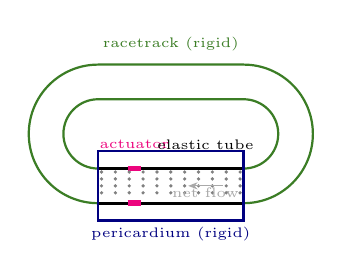
\begin{tikzpicture}[scale=4.4]
  % racetrack: outer and inner
  \draw[OliveGreen,thick] (-0.21,0.2) -- (0.21,0.2) arc (90:-90:0.2) -- (-0.21,-0.2) arc (270:90:0.2);
  \draw[OliveGreen,thick] (-0.21,0.1) -- (0.21,0.1) arc (90:-90:0.1) -- (-0.21,-0.1) arc (270:90:0.1);
  % elastic tube (bottom straight section) over the racetrack's bottom
  \draw[black,very thick] (-0.21,-0.1) -- (0.21,-0.1); \draw[black,very thick] (-0.21,-0.2) -- (0.21,-0.2);
  % pericardium
  \draw[NavyBlue,thick] (-0.21,-0.05) rectangle (0.21,-0.25);
  % actuator (a quarter along)
  \draw[RubineRed,line width=2pt] (-0.125,-0.1) -- (-0.085,-0.1); \draw[RubineRed,line width=2pt] (-0.125,-0.2) -- (-0.085,-0.2);
  % markers
  \foreach \x in {-0.2,-0.16,...,0.2}{\foreach \y in {-0.11,-0.13,...,-0.19}{\fill[gray] (\x,\y) circle (0.15pt);}}
  \node[font=\tiny,text=OliveGreen] at (0,0.26) {racetrack (rigid)};
  \node[font=\tiny,text=NavyBlue] at (0,-0.29) {pericardium (rigid)};
  \node[font=\tiny,text=RubineRed] at (-0.105,-0.03) {actuator};
  \node[font=\tiny] at (0.1,-0.03) {elastic tube};
  \draw[-{Stealth[length=1.2mm]},DarkGray] (0.15,-0.15) -- (0.05,-0.15); \node[font=\tiny,text=DarkGray] at (0.1,-0.17) {net flow};
\end{tikzpicture}

\scriptsize The loop, redrawn from the 2014 slide: a $1$ m box; tube diameter $0.1$ m; inner radius of the bends $0.1$ m; pericardium $0.2$ m across; actuator $0.04$ m long, centred a quarter of the way along the elastic section. Chapter 36 derives the geometry for the two-point pump. The arrow is the net flow along the elastic section measured in both suction modes (chapter 29).
\end{column}
\end{columns}
\end{frame}

% 14
\begin{frame}[fragile]{The generator and the input: parts, numbers, order}
\label{fr:parts}
\vspace{-1mm}
\begin{columns}[T,onlytextwidth]
\begin{column}{0.5\textwidth}
\begin{lstlisting}[style=inputtiny]
// input2d (mode TARGET_VP): the driving pieces first
ACTUATION = "TARGET_VP"
FRE = 1.0                      // pumping frequency (Hz)
WO  = 10.0                     // Womersley number
MU  = 2.0*PI*FRE*RHO*D*D/(4.0*WO*WO)   // 0.157 N s/m^2
...
IBStandardInitializer {
   max_levels = MAX_LEVELS
   structure_names = "actuator_top_512", "actuator_bot_512",
                     "heart_tube_512", "heart_peri_512",
                     "heart_race_512", "markers_512"
   ...
}
\end{lstlisting}
\scriptsize ``Note on order: in \code{input2d} the actuator (one of \code{actuator\_top/bot}, \code{vp\_aforce}, \code{peri\_aforce}) must be first under \code{structure\_names}'' (2014): the update functions ask for structure 0 (and 1). Five input files, one per mode, differ only in \code{ACTUATION} and this list; \code{make\_inputs.py} writes the other four from \code{input2d}.
\end{column}
\begin{column}{0.48\textwidth}
\footnotesize The driven points of the actuators are \al{copies} of points of the tube: each actuator structure holds its own vertices at the same places, and the tube's points there stay ordinary elastic points. A tether or an applied force on the copy moves the fluid of those grid cells, and the tube's wall goes with it. This is why the counts of the tube (860) do not change between modes, and why the input lists the driving pieces as separate structures.
\vspace{1mm}

\footnotesize Stiffnesses: $K = 2$, $EI = 10^{-2}$, $\kappa = 2$ (file values $2048$, $1.07\times10^7$, $2048$); $F_{\mathrm{mag}} = 0.25$ for the suction force and $1$ for the travelling one (the 2014 code's $4$, ``my best guess at a reasonable applied force'', closes the tube: slide \ref{fr:fmag}). The fluid: $\rho = 1000$, $\mu = 0.157$ from $\mathrm{Wo} = 10$ at $f = 1$ Hz.
\end{column}
\end{columns}
\end{frame}

% 14b
\begin{frame}{The generator: parts and numbers}
\label{fr:parts2}
\begin{columns}[T,onlytextwidth]
\begin{column}{0.5\textwidth}
\scriptsize
\setlength{\tabcolsep}{3pt}
\begin{tabular}{@{}L{0.41\textwidth}L{0.31\textwidth}r@{}}
\toprule
structure & files & points\\
\midrule
\code{heart\_tube\_512} & vertex, spring (858), beam (856), target (40) & 860\\
\code{heart\_tube\_stiff\_512} & the same, beams $\times 10$ (mode 3) & 860\\
\code{heart\_race\_512} & vertex, target & 3436\\
\code{heart\_peri\_512} & vertex, target & 1066\\
\code{markers\_512} & vertex only & 121\\
\code{actuator\_top/\allowbreak bot\_512} & vertex, target & $2\times41$\\
\code{pperi\_top/\allowbreak bot\_512} & vertex, target & $2\times308$\\
\code{vp\_aforce\_512} & vertex, spring (41, index 1) & 82\\
\code{peri\_aforce\_512} & vertex, spring (328, index 2) & 656\\
\code{peri\_kwave\_512} & vertex, spring (328, index 0) & 656\\
\bottomrule
\end{tabular}

\end{column}
\begin{column}{0.48\textwidth}
\footnotesize ``The MATLAB code generates each of the boundaries with parameters specified towards the beginning of the code. Note that $N = 512$ assumes the fluid is solved on a $512\times512$ grid. If $L$ is the length of the domain, then the distance between the boundary points must be close to $L/(2N)$.'' (2014)
\vspace{1mm}

\footnotesize The Python generator \code{generate\_mesh2d.py} is a line-by-line port of the 2014 MATLAB one (shipped too, with a few edits) and writes the same 27 files token for token. The geometry its parameters set: a $1$ m box; tube diameter $0.1$ m; straight sections $0.42$ m (elastic part $0.4$ m plus ten rigid points at each end); bends of inner radius $0.1$ m; pericardium $0.2$ m across; points $\Delta s = L/(2N) = 1/1024$ m apart, half a grid cell.
\end{column}
\end{columns}
\end{frame}

% 15
\begin{frame}[fragile]{Mode 1: dynamic suction pumping with target points}
\label{fr:targetvp}
\begin{columns}[T,onlytextwidth]
\begin{column}{0.52\textwidth}
\begin{lstlisting}[style=cpptiny]
// update_target_point_positions.cpp (IB/11), the motion
const double squeeze = (pump::amp / 2.0) * (1.0 + std::sin(2.0 * M_PI * freq * current_time - M_PI / 2.0));
...
if (actuator_top_idxs.first <= lag_idx && lag_idx < actuator_top_idxs.second)
    X_target[1] = -pump::R2 - squeeze;   // the top wall, at y = -R2, moves down
if (actuator_bot_idxs.first <= lag_idx && lag_idx < actuator_bot_idxs.second)
    X_target[1] = -pump::R1 + squeeze;   // the bottom wall, at y = -R1, moves up
\end{lstlisting}
\footnotesize \code{amp} $= 0.8\times$ diameter$/2$: at full squeeze the walls are $20\%$ of the diameter apart. The targets are \al{set} to a position computed from the time (chapter 9a's second form), so the motion is the same whatever \code{DT} is and survives a restart.
\end{column}
\begin{column}{0.46\textwidth}
\footnotesize ``How to turn on VP with target points: in \code{main.C}, uncomment \code{update\_target\_point\_positions} and comment out \code{update\_springs\_vp\_aforce} / \code{update\_springs\_peri\_aforce}.'' (2014) In IB/11 that is \code{ACTUATION = "TARGET\_VP"}, and \code{main.cpp} calls the matching function:
\begin{lstlisting}[style=cpptiny]
if (actuation == "TARGET_VP")
    update_target_point_positions(patch_hierarchy, l_data_manager, loop_time, dt, freq);
else if (actuation == "FORCE_VP")
    update_springs_vp_aforce(patch_hierarchy, l_data_manager, loop_time, dt, freq);
...
\end{lstlisting}
\footnotesize Why it pumps: the squeeze is not in the middle of the elastic section, so the two sides of the tube respond differently to it (one is nearer the rigid racetrack); the asymmetry makes a net flow round the loop. This is Liebau's valveless pumping, which chapter 36 studies with two pumps.
\end{column}
\end{columns}
\end{frame}

% 16
\begin{frame}{``Things you might want to change''}
\label{fr:change}
\small The 2014 lecture's list, kept, with where each change lives in IB/11:
\vspace{1mm}

\scriptsize
\begin{tabular}{@{}L{0.3\textwidth}L{0.3\textwidth}L{0.32\textwidth}@{}}
\toprule
Change & 2014 & IB/11\\
\midrule
the diameter & \code{generate\_mesh2d.m} and \code{update\_target\_point\_\allowbreak positions.C} & the generator and \code{pump\_geometry.h} (one header the update functions share)\\
removing the racetrack or pericardium & remove them from \code{structure\_names} & the same\\
$\mathrm{Wo}$, by changing the viscosity & \code{input2d} & \code{WO} in the input; $\mu$ follows\\
the pumping frequency & \code{input2d} and the update file & \code{FRE} in the input only (passed to the update functions)\\
the location or width of the actuator & \code{generate\_mesh2d.m} & the generator (\code{La}, \code{Ca})\\
material properties & \code{generate\_mesh2d.m} & the generator (\code{kappa\_spring}, \code{kappa\_beam}, \code{kappa\_target})\\
the force magnitude (``which will change the amplitude of contraction'') & \code{generate\_mesh2d.m} & the generator (\code{Fmag}, written into the \code{.spring} files)\\
the width and speed of the peristaltic packet & hard-coded in the update files & \code{PERI\_WIDTH}, \code{PERI\_SPEED} in the input\\
\bottomrule
\end{tabular}

\vspace{1mm}
\footnotesize Two numbers are repeated between files by design and must agree: the diameter and the point spacing (generator and header), and the actuator's index range (the generator's \code{Na1}, \code{Na2} and the structure order in the input). Chapter 8a's rule: change one thing, rerun the generator, check the counts in the log.
\end{frame}

% 17
\begin{frame}[fragile]{Mode 2: the same pump by an applied force}
\label{fr:forcevp}
\begin{columns}[T,onlytextwidth]
\begin{column}{0.5\textwidth}
\footnotesize ``Part 2: create your own force. Goal: we want to drive the motion of the tube by adding an external force to the boundary. Application 1: valveless suction pumping with applied force. Let's create a simple applied sinusoidal force of the form $F = F_{\mathrm{mag}}(1 + \sin(2\pi f t - \pi/2))$.'' (2014)
\begin{lstlisting}[style=cpptiny]
// main.cpp (IB/11): the force function, registered under indices 1 and 2
inline double applied_force(double /*R*/, const double* params, int, int)
{
    const double F = params[0];          // Fmag, from the .spring file
    const double phase_fun = params[1];  // set every step by the update function
    return F * phase_fun;
}
\end{lstlisting}
\begin{lstlisting}[style=cpptiny]
// update_springs_vp_aforce.cpp (IB/11): the phase for this step
const double phase = 0.5 * (1.0 + std::sin(2.0 * M_PI * freq * current_time - M_PI / 2.0));
...
for (std::vector<double>& spring : spring_spec->getParameters())
    spring[1] = phase;
\end{lstlisting}
\end{column}
\begin{column}{0.48\textwidth}
\scriptsize The structure \code{vp\_aforce\_512}: the actuator's $41 + 41$ points, with a ``spring'' from each top point $i$ to the bottom point $i + 41$ under it, parameters $F_{\mathrm{mag}}$ and phase, index 1 (slide \ref{fr:column}). ``Note that we are modifying the phase and not the $F_{\mathrm{mag}}$.''
\begin{itemize}
  \item the tension $F_{\mathrm{mag}}\cdot\mathrm{phase}$ pulls each pair of wall points together: a force across the tube, zero when the phase is zero;
  \item the 2014 code's phase is $\frac12(1 + \sin)$, between 0 and 1, the lecture's $1 + \sin$ between 0 and 2; IB/11 uses the code's;
  \item unlike mode 1, the walls are not told where to go: ``depending on the choice of $F_{\mathrm{mag}}$, the contraction may be too much or too little. You will need to tune it as you change parameters.'' The 2014 value, $4$, closed the tube at $0.24$ s and the pinch slid along the tube; $2$ closed it at $0.32$ s, $1$ at $0.44$ s, $0.5$ in its second squeeze; IB/11 ships $0.25$ (slides \ref{fr:fmag}, \ref{fr:fmag2}).
\end{itemize}
\scriptsize ``The pieces are the same as the valveless pump driven by target points. A sinusoidal force is applied in the same region.''
\end{column}
\end{columns}
\end{frame}

% 18
\begin{frame}[fragile]{Mode 3: peristalsis by a travelling force}
\label{fr:forceperi}
\begin{columns}[T,onlytextwidth]
\begin{column}{0.52\textwidth}
\footnotesize ``Application 2: peristalsis with applied force. We will model the dynamics of the force as a Gaussian wave packet, $\mathrm{phase} = \exp(-(x - x_c)^2/w^2)$, where $x_c$ is the center of the Gaussian, $w$ is the width. $x_c$ travels with $ct$, where $c$ is the wave speed and $t$ is time. We will determine the time since the beginning of the pulse using time $-$ floor(time/period)$\cdot$period; the pulse number is floor(time/period).'' (2014, and the June 2014 note)
\begin{lstlisting}[style=cpptiny]
// update_springs_peri_aforce.cpp (IB/11)
const double period = 1.0 / freq;
const double ww = peri_width;                      // width of the packet (m): PERI_WIDTH in the input
const double speed = peri_speed * lperi / period;  // wave speed (m/s): PERI_SPEED piece lengths per period
const int pulse_number = static_cast<int>(std::floor(current_time / period));
const double pulse_time = current_time - pulse_number * period;
const double xc = speed * pulse_time - 0.15 * lperi;
...
const double x = (lag_idx - muscle_idxs.first) * pump::ds;   // the spring's position
const double phase = std::exp(-(x - xc) * (x - xc) / (ww * ww));
for (std::vector<double>& spring : spring_spec->getParameters()) spring[1] = phase;
\end{lstlisting}
\end{column}
\begin{column}{0.46\textwidth}
\scriptsize The structure \code{peri\_aforce\_512}: the middle $0.32$ m of the tube, $328 + 328$ points, springs across the tube with $F_{\mathrm{mag}}$, phase and index 2. One packet per period starts just before the piece and runs along it at \code{PERI\_SPEED} piece lengths per period; where it is, the walls are pulled together; the squeeze travels and pushes the fluid ahead of it.
\vspace{1mm}

\scriptsize What the 2014 slides had, and what IB/11 fixes: next slide.
\end{column}
\end{columns}
\end{frame}

% 18b
\begin{frame}{Mode 3 (2): what the 2014 slides had, and what IB/11 fixes}
\label{fr:forceperi2}
\footnotesize
\begin{itemize}
  \item \al{An undefined variable.} The lecture's loop over previous pulses used a variable \code{c} that was never defined (it meant \code{speed}), and it added the packets of all earlier pulses, which had long left the piece. One packet per period is the same thing, and is what IB/11 does.
  \item \al{Hard-coded width and speed.} The lecture's width and speed were $0.025$ m and $1.0$ piece length per period, the code's $0.005$ m and $1.3$, both hard-coded. IB/11 reads them from the input (\code{PERI\_WIDTH}, \code{PERI\_SPEED}) and ships the lecture's width with the code's speed, because the $5$ mm packet with $F_{\mathrm{mag}} = 4$ closed the tube completely at the first pinch (slide \ref{fr:wrong2}).
  \item \al{A stiffer tube for this mode.} IB/11 runs the force-driven wave on a tube ten times stiffer in bending (\code{heart\_tube\_stiff\_512}, $EI = 0.1$, at $\Delta t = 2.5\times10^{-5}$), because with the 2014 tube the fluid the packet pushes ahead piles up and the slack tube behind the packet collapses and sticks, whatever the force (slides \ref{fr:fmag}, \ref{fr:fmag2}).
  \item \al{A harmless slip.} The lecture's slide 33 registered index 2 with the \emph{VP} function; the two functions are identical, so nothing changed.
\end{itemize}
\end{frame}

% 19
\begin{frame}[fragile]{Mode 4: the 2014 code's peristalsis, a travelling stiffness}
\label{fr:kwave}
\begin{columns}[T,onlytextwidth]
\begin{column}{0.52\textwidth}
\scriptsize The lecture described the force version; the code the lab actually ran in 2014 did something cleverer with the \emph{default} spring: \code{peri\_kwave\_512.spring} has springs across the tube with stiffness $0$ and rest length $(1 - \mathrm{percont})\times$ diameter (the 2014 code's \code{percont} $= 0.8$ gave $0.02$ m; IB/11 ships $0.5$, $0.05$ m: slide \ref{fr:wrong2}), index 0, and the update function sets each spring's \emph{stiffness} to a travelling Gaussian:
\begin{lstlisting}[style=cpptiny]
// update_springs_peri_kwave.cpp (IB/11)
const double kmax = (kappa_spring / 10.0) / pump::ds;   // 102.4 in file units
...
const double stiffness = kmax * std::exp(-(x - xc) * (x - xc) / (ww * ww));
for (std::vector<double>& spring : spring_spec->getParameters()) spring[0] = stiffness;
\end{lstlisting}
\scriptsize Where the packet is, the springs are stiff and pull the walls toward the rest length; elsewhere they are slack. Hooke's law does the rest. The packet's width and speed are \code{PERI\_WIDTH} and \code{PERI\_SPEED}, as in mode 3, and the same taper at the piece's ends applies.
\end{column}
\begin{column}{0.46\textwidth}
\scriptsize Force or stiffness?
\begin{itemize}
  \item an \al{applied force} does not know when to stop: with $F_{\mathrm{mag}}$ too large the walls meet and cross, and the 2014 \code{main.C} added an ad-hoc penalty to its peristaltic force (\code{F*(phase - 1/(R*512/4)\^{}2)}, ``a penalty that will hopefully stop the boundaries from getting too close'');
  \item a \al{stiffness wave} with a rest length is bounded by construction: the squeeze cannot go past the rest length, and $k_{\max}$ sets how hard it tries. The price is that the contraction amplitude depends on the tube's own stiffness and the fluid, like a muscle's does;
  \item a \al{target wave} (next slide) is exact and bounded, but it is kinematics, not a force: the walls go where they are told whatever the fluid does.
\end{itemize}
\scriptsize All three are ``your own force'' in the sense of this chapter; the parameters they change are different slots of the same spring.
\end{column}
\end{columns}
\end{frame}

% 20
\begin{frame}[fragile]{Mode 5: prescribed peristalsis with target points}
\label{fr:targetperi}
\begin{columns}[T,onlytextwidth]
\begin{column}{0.52\textwidth}
\begin{lstlisting}[style=cpptiny]
// update_target_point_positions_peri.cpp (IB/11)
const double s_ramp = 0.5 / freq;                                     // ramp over half a period
const double c_amp = (current_time < s_ramp) ? current_time / s_ramp : 1.0;
const double L_taper = 0.05;                                          // the wave dies out over 5 cm at each end
auto envelope = [&](double s) { ... raised cosine from 0 to 1 over L_taper, mirrored at Lap ... };
...
const double s = (lag_idx - top_idxs.first) * pump::ds;               // position along the piece (m)
const double wave = std::sin(-2.0 * M_PI * freq * current_time + 2.0 * M_PI * (s / pump::Lap));
X_target[1] = -pump::R2 - pump::amp * c_amp * envelope(s) * wave;     // top wall
...
X_target[1] = -pump::R1 + pump::amp * c_amp * envelope(s) * wave;     // bottom wall
\end{lstlisting}
\scriptsize The structures \code{pperi\_top/bot\_512}: the middle $0.3$ m of each wall, every point a target. One sine wavelength fits the piece and travels to the right at $f$ wavelengths per second; the crest narrows the tube to $20\%$, the trough widens it into the pericardium's gap.
\end{column}
\begin{column}{0.46\textwidth}
\scriptsize This is the \code{update\_target\_point\_positions\_peri} of the 2014 \code{Forced-tube-pump} code, which its \code{main.C} was calling when the folder was archived (with the other three calls commented out), plus the taper. Compared with mode 1 it is a longer piece with a wave instead of a uniform squeeze; compared with modes 3 and 4 it prescribes the shape instead of a force.
\begin{itemize}
  \item the ramp \code{c\_amp} avoids the impulsive start of chapter 7;
  \item the \al{taper} is new: the 2014 wave did not vanish at the ends of the piece, so the last driven point stood up to $4$ cm proud of the first free point of the wall one spacing away, and the run aborted at $t = 0.77$ s (slide \ref{fr:wrong2});
  \item \code{Lap} $= 0.3$ m is the wavelength; the 2014 file called it \code{Let}, which in the generator is the elastic tube's length ($0.4$ m), a name clash IB/11 removes;
  \item the amplitude is a position, so this mode has no $F_{\mathrm{mag}}$ to tune and no risk of crossing walls, and the force it needs is whatever the tethers must supply.
\end{itemize}
\end{column}
\end{columns}
\end{frame}

% 21
\begin{frame}{The five modes in one table}
\label{fr:modes}
\scriptsize
\setlength{\tabcolsep}{3pt}
\begin{tabular}{@{}L{0.14\textwidth}L{0.17\textwidth}L{0.2\textwidth}L{0.2\textwidth}L{0.2\textwidth}@{}}
\toprule
mode & driving structure & what is set each step & force law & what is prescribed\\
\midrule
\code{TARGET\_VP} & \code{actuator\_top/bot} (2 structures) & target positions & tether (target point) & the walls' positions at one spot\\
\code{FORCE\_VP} & \code{vp\_aforce} & \code{params[1]} = phase & index 1: $F_{\mathrm{mag}}\cdot$phase & a force across the tube at one spot\\
\code{FORCE\_PERI} & \code{peri\_aforce} & \code{params[1]} = travelling Gaussian & index 2: $F_{\mathrm{mag}}\cdot$phase & a travelling force\\
\code{STIFFNESS\_PERI} & \code{peri\_kwave} & \code{params[0]} = travelling stiffness & index 0: $k(x,t)\,(R - 0.05)$ & a travelling pull toward 50\% opening\\
\code{TARGET\_PERI} & \code{pperi\_top/bot} (2 structures) & target positions & tether & a travelling wall shape\\
\bottomrule
\end{tabular}

\vspace{2mm}
\small The same tube, pericardium, racetrack and markers in all five; the same \code{main.cpp}, which dispatches on \code{ACTUATION}; one input file each. The next slides show what the five do in two periods.
\vspace{1mm}

\small Run times are in the README; four modes run at \code{DT = 5e-5} (the course's \code{1e-5} was a safe choice for a 10 s run; chapter 8a's rule puts the limit between the two for these stiffnesses), and \code{FORCE\_PERI}, on its ten-times-stiffer tube, at \code{2.5e-5}.
\end{frame}

% 22
\begin{frame}{What the five modes do: transport and squeeze}
\label{fr:transport}
\begin{columns}[T,onlytextwidth]
\begin{column}{0.6\textwidth}
\centering
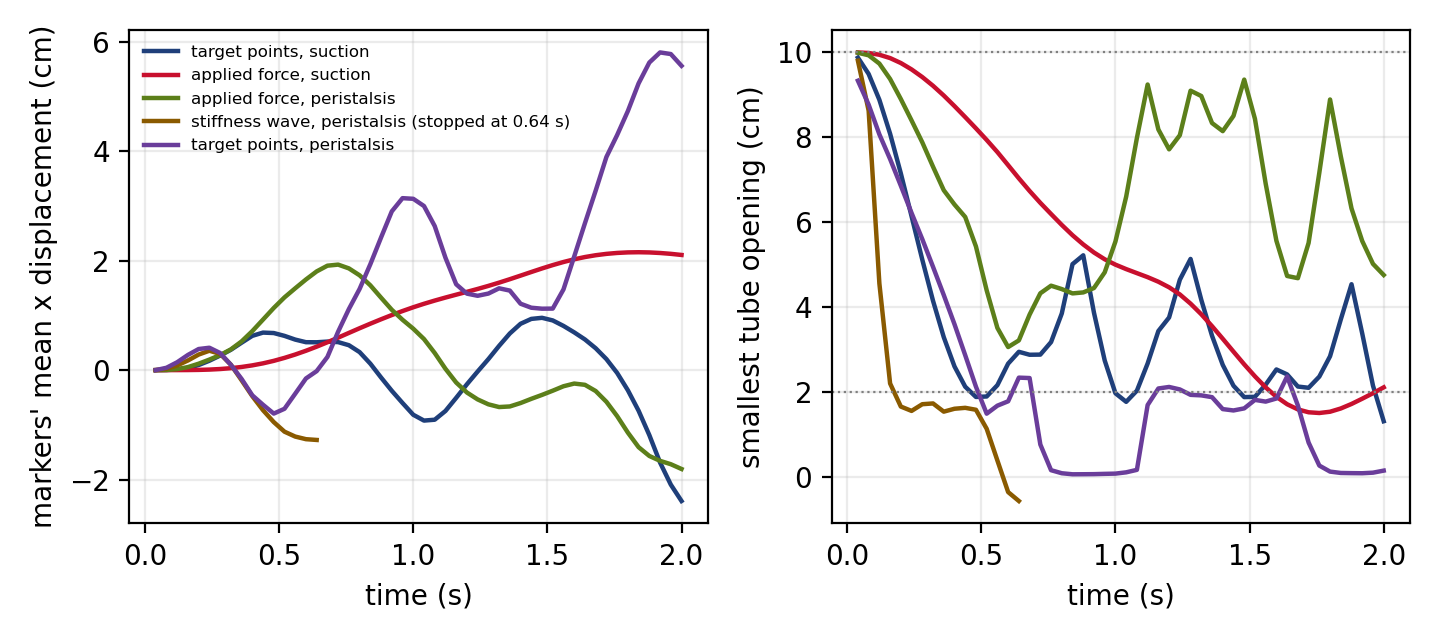
\includegraphics[width=\textwidth]{ch9b-pump-transport}
\end{column}
\begin{column}{0.38\textwidth}
\footnotesize Left: the mean $x$-position of the 121 markers, which start inside the elastic section, against time: how far those parcels drift along the tube, which is not always the direction of the net flow round the loop (next slide). Right: the smallest opening of the elastic section against time: how hard each mode squeezes (the diameter is $10$ cm; the suction targets close to $2$ cm by construction, and the 2014 target wave closes the tube and reopens it).
\vspace{1mm}

\footnotesize The numbers are in the README and on slide \ref{fr:fmag2} (two periods, shipped parameters; a curve that ends early ends where its run stopped). What to look for: next slide.
\end{column}
\end{columns}
\sourcecredit{IB/11 with IBAMR 0.19.0, the five input files as shipped, 2 s each; \code{tools/ch9b\_figures.py} reads \code{hier\_data\_IB2d/X.*} (the structures in input order; the markers last).}
\end{frame}

% 22b
\begin{frame}{What the five modes do: what to look for}
\label{fr:lookfor}
\footnotesize
\begin{itemize}
  \item The target-driven modes squeeze as told, and the elastic walls between the tethered copies go a little further.
  \item The applied-force modes squeeze as far as $F_{\mathrm{mag}}$ can push against the tube and the fluid, and nothing tells them when to stop (slide \ref{fr:fmag}).
  \item The markers' drift has a direction, and it depends on the squeeze: the target-driven suction pump sends the markers toward the nearer end of the elastic section ($-2.4$ cm in two periods); the force-driven one, which squeezes less and later, sends them the other way ($+2.1$ cm); the target wave sends them with the wave ($+5.6$ cm); the force-driven wave on the stiff tube sloshes them back and forth ($+0.8$, then $-2.6$ cm). The net flow round the loop, integrated across the tube from the velocity (chapter 29), turns the same way in both suction modes: clockwise, $-x$ along the elastic section, $1.6 \times 10^{-3}$ m$^2$/s with the targets and $6.7 \times 10^{-4}$ with the applied force (two-period means); the force-driven markers drift against it.
  \item The target-driven suction pump's smallest opening in its second period ($1.3$ cm at $t = 2$ s) is beside the actuator, not in it: the actuator has reopened and sucks the neighbouring elastic wall in, which is what ``dynamic suction'' means (slide \ref{fr:shapes}, top right).
  \item The net flow per period is the figure of merit of a pump; measure it from the velocity across the tube (chapter 29). It depends on the wall motion achieved and its timing, not on how the motion was produced: the same wall motion gives the same flow, and the five modes achieve five different motions (slide \ref{fr:fmag2}).
\end{itemize}
\end{frame}

% 23
\begin{frame}{What the five modes do: the tube at full squeeze}
\label{fr:shapes}
\begin{columns}[T,onlytextwidth]
\begin{column}{0.58\textwidth}
\centering
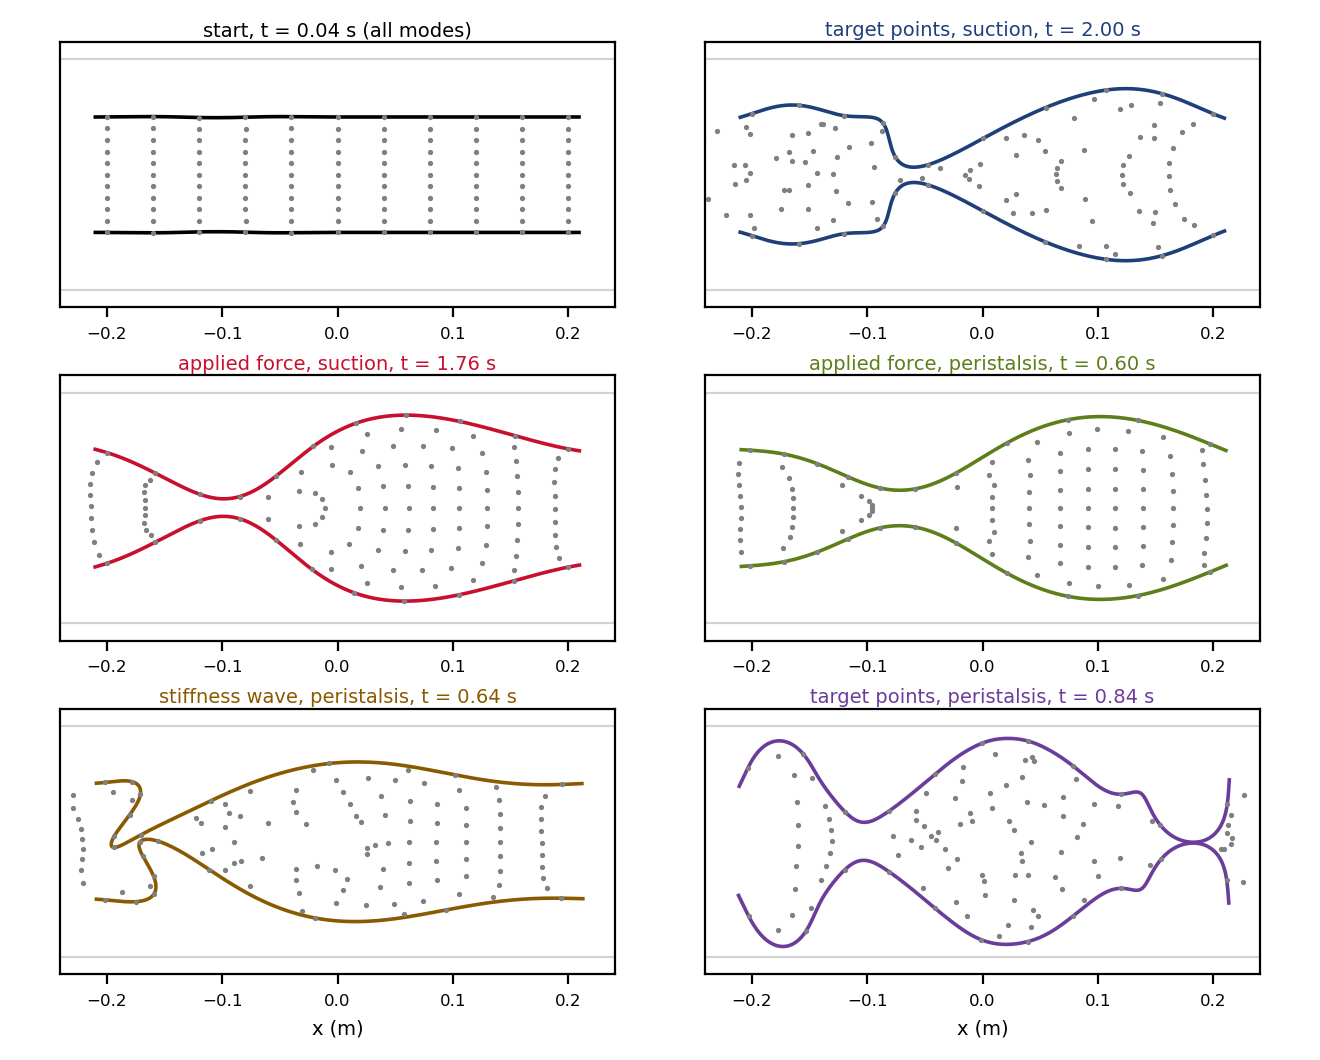
\includegraphics[height=0.72\textheight]{ch9b-pump-shapes}
\end{column}
\begin{column}{0.4\textwidth}
\scriptsize The elastic section (both walls), the pericardium's walls (grey lines) and the markers (grey dots) at the start and at the moment of the smallest opening in each mode.
\begin{itemize}
  \item the suction modes (1, 2) pinch one spot a quarter of the way along; the elastic walls around the pinch bulge;
  \item the peristaltic modes (3, 4, 5) show the travelling constriction and, ahead of it, the bulge of fluid it pushes;
  \item the markers' positions show where those 121 parcels have gone since $t = 0$ (not the net flow, chapter 29); compare the panels with the curves of slide \ref{fr:transport}.
\end{itemize}
\scriptsize The 2014 slides showed the same two pictures from VisIt (``VP with applied force'', ``Results from peristalsis''), with velocity vectors; chapter 26's recipe reproduces them from \code{viz\_IB2d}, and the README has one.
\end{column}
\end{columns}
\sourcecredit{Same runs; \code{tools/ch9b\_figures.py}.}
\end{frame}

% 23b
\begin{frame}{Tuning the applied force}
\label{fr:fmag}
\begin{columns}[T,onlytextwidth]
\begin{column}{0.6\textwidth}
\centering
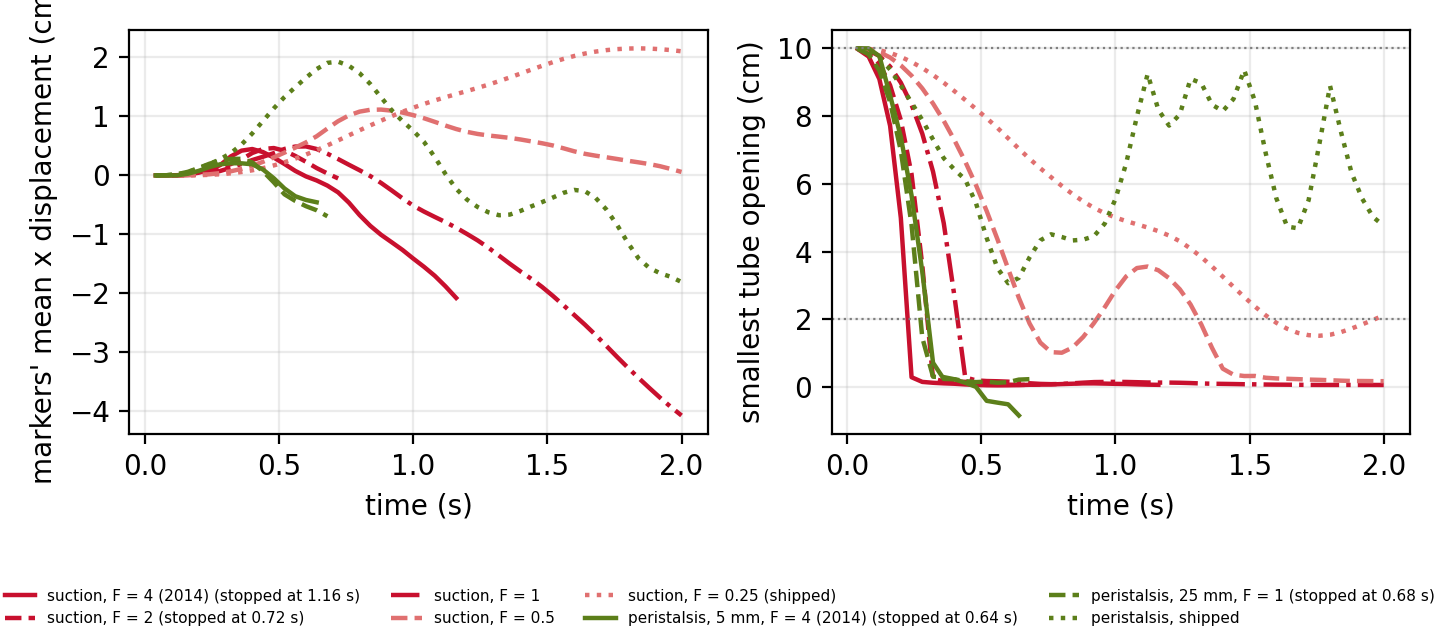
\includegraphics[width=\textwidth]{ch9b-pump-fmag}
\end{column}
\begin{column}{0.38\textwidth}
\footnotesize The two applied-force modes at the 2014 values and at the shipped ones: the markers' transport (left) and the smallest opening (right). Solid: the 2014 code's $F_{\mathrm{mag}} = 4$ (suction) and its $5$ mm packet with $F_{\mathrm{mag}} = 4$ (peristalsis); dashed and dotted: smaller forces, the lecture's $25$ mm packet, the stiffer tube.
\vspace{1mm}

\footnotesize Shipped: the largest forces tried that do not close the tube in two periods, $0.25$ for the actuator and $1$ for the $25$ mm packet on the stiffer tube; every run's numbers are on the next slide.
\vspace{1mm}

\scriptsize ``You will need to tune it as you change parameters'' (2014) is the whole of this slide: an applied force has no notion of the shape it should produce, and the first run with a new $F_{\mathrm{mag}}$ is a measurement of what it does.
\end{column}
\end{columns}
\sourcecredit{IB/11, IBAMR 0.19.0; runs that stopped at the CFL limit are marked with the time they reached; \code{tools/ch9b\_figures.py}.}
\end{frame}

% 23c
\begin{frame}{Tuning the applied force: the numbers}
\label{fr:fmag2}
\scriptsize Every applied-force run of the chapter, from the saved positions. ``Closes'': the walls come within two grid cells ($0.4$ cm; $\Delta x = 0.195$ cm), share cells and stick. Drift: the markers' mean displacement over $0$--$1$ s and over $1$--$2$ s (not the net flow, chapter 29). Opening: the smallest wall-to-wall distance in each period.
\par\smallskip{\centering\scriptsize\renewcommand{\arraystretch}{0.96}
\begin{tabular}{@{}llllll@{}}
\toprule
run & tube & closes at & run ends & markers' drift (cm) & opening (cm)\\
\midrule
suction, $F_{\mathrm{mag}} = 4$ (2014) & 2014 & $0.24$ s & abort, $1.16$ s & $-1.4$ & $0.05$\\
suction, $2$ & 2014 & $0.32$ s & abort, $0.72$ s & -- & $0.07$\\
suction, $1$ & 2014 & $0.44$ s & $2$ s & $-0.5$, $-3.6$ & $0.09$, $0.06$\\
suction, $0.5$ & 2014 & $1.44$ s & $2$ s & $+1.0$, $-1.0$ & $1.0$, $0.17$\\
suction, $0.25$ (shipped) & 2014 & never & $2$ s & $+1.1$, $+1.0$ & $5.0$, $1.5$\\
peristalsis, $5$ mm, $4$ (2014) & 2014 & $0.36$ s & abort, $0.64$ s & -- & crossed\\
peristalsis, $25$ mm, $1$ & 2014 & $0.32$ s & abort, $0.68$ s & -- & $0.13$\\
peristalsis, $25$ mm, $1$ (shipped) & $10\times EI$ & never & $2$ s & $+0.8$, $-2.6$ & $3.1$, $4.7$\\
\midrule
target points, suction & 2014 & never & $2$ s & $-0.8$, $-1.6$ & $1.9$, $1.3$\\
target points, peristalsis & 2014 & $0.76$ s, reopens & $2$ s & $+3.1$, $+2.4$ & $0.07$, $0.09$\\
stiffness wave, $25$ mm, rest $5$ cm & 2014 & $0.56$ s & abort, $0.64$ s & -- & crossed\\
\bottomrule
\end{tabular}\par}\vspace{1pt}
\scriptsize Two things to read off. The shipped suction force pumps steadily (its net flow never reverses) and turns the loop the same way as the target-driven pump, though its markers drift the other way (chapter 29). Its squeeze is shallower and lags the force by half a period ($5.0$ cm at $t = 1.0$ s for a force that peaked at $0.5$ s). The force-driven wave on the stiff tube runs but sloshes: the fluid it pushes ahead flows back when the packet leaves the piece, and two periods do not settle its direction; a larger $F_{\mathrm{mag}}$ on the stiff tube is the first thing to try (slide \ref{fr:hw}).
\sourcecredit{Same runs; \code{tools/ch9b\_figures.py} prints these numbers.}
\end{frame}

% 24
\begin{frame}{Measuring a pump: the pump coefficient}
\label{fr:cpump}
\small From the 2014 lecture, ``Analysis -- pump coefficient'': ``The pump coefficient is given by $C_{\mathrm{pump}} = m\,U_a^2/W$, where $m$ is the total mass of fluid in the loop, $U_a$ is the average fluid velocity in the direction of the loop, and $W$ is the total work done by the pump over a set period of time. Note that work is $F\cdot d$, and we calculate each of these in IBM.''
\begin{itemize}
  \item $m = \rho\,A_{\mathrm{loop}}$ per unit depth, from the geometry;
  \item $U_a$ from the velocity field integrated across the tube: the flux divided by the diameter (chapter 29); not from the markers' displacement, which can differ even in sign (slide \ref{fr:lookfor});
  \item $W = \sum_{\text{steps}}\sum_{\text{driven points}} \mathbf{F}_k\cdot\Delta\mathbf{X}_k$: the force on each driven point times its displacement, summed over a period, from the \code{F.*} and \code{X.*} files (chapter 11). For the target modes the force is the tether force; for the force modes it is $F_{\mathrm{mag}}\cdot$phase on each spring, which \code{F.*} also contains.
\end{itemize}
\vspace{1mm}
\begin{punchbox}
\small $C_{\mathrm{pump}}$ is a kinetic energy over a work: the fraction of the pump's effort that ends up moving the whole loop. It is one of chapter 8b's dimensionless outputs, and the quantity the valveless-pump studies of Part VI compare across frequencies, $\mathrm{Wo}$ and actuator positions.
\end{punchbox}
\end{frame}

% 25
\begin{frame}[fragile]{Other laws you can write}
\label{fr:laws}
\begin{lstlisting}[style=cpptiny]
// a spring that only pulls (a cable, a tendon): slack under compression
inline double cable_force(double R, const double* params, int, int)
{   const double k = params[0], r0 = params[1];
    return (R > r0) ? k * (R - r0) : 0.0; }
// a stiffening (cubic) tissue spring: three numbers per line of the .spring file
inline double cubic_force(double R, const double* params, int, int)
{   const double k = params[0], r0 = params[1], k3 = params[2], e = R - r0;
    return k * e + k3 * e * e * e; }
// a muscle: passive spring plus an active tension that the update function writes into params[2]
inline double muscle_force(double R, const double* params, int, int)
{   const double k = params[0], r0 = params[1], T_active = params[2];
    return k * (R - r0) + T_active; }
\end{lstlisting}
\begin{columns}[T,onlytextwidth]
\begin{column}{0.48\textwidth}
\scriptsize The pattern is always the same: a tension from $R$ and the parameters; anything that varies in time or along the fibre arrives through a parameter that the update function writes.
\begin{itemize}
  \item a \al{force--length} muscle law: make \code{T\_active} depend on $R$ too, e.g.\ a Gaussian in $R/r_0$ about its optimum;
  \item a \al{force--velocity} law needs the velocity, which a spring function does not get; use a Lagrangian force strategy (next slide) or store the previous length in a parameter and difference it;
\end{itemize}
\end{column}
\begin{column}{0.48\textwidth}
\scriptsize
\begin{itemize}
  \item IB2d (chapter 4e) ships muscle models of exactly these forms, which is a good place to test a law before writing it in C++;
  \item give each law its own index and its own generator loop, and write the derivative or pass \code{nullptr}.
\end{itemize}
Chapter 10 does the same for beams (a preferred curvature that changes in time makes a fin flap); chapter 36 drives a tube with two such muscles out of phase.
\end{column}
\end{columns}
\end{frame}

% 26
\begin{frame}[fragile]{Beyond springs: three other ways to put a force on a structure}
\label{fr:other}
\begin{lstlisting}[style=cpptiny]
// 1. A Lagrangian force strategy of your own (IBLagrangianForceStrategy.h): the whole force on every point
class MyForce : public IBLagrangianForceStrategy
{   void computeLagrangianForce(Pointer<LData> F_data, Pointer<LData> X_data, Pointer<LData> U_data,
                                Pointer<PatchHierarchy<NDIM>> hierarchy, int level_number,
                                double data_time, LDataManager* l_data_manager) override;  ... };
// several strategies at once (yours and the standard one): IBLagrangianForceStrategySet(begin, end)
ib_method_ops->registerIBLagrangianForceFunction(new IBLagrangianForceStrategySet(v.begin(), v.end()));
// 2. A uniform body force on one structure (IBStandardForceGen.h); F is an IBTK::Vector
ib_force_fcn->setUniformBodyForce(F, structure_id, level_number);
// 3. An Eulerian body force on the fluid (chapter 7): the ForcingFunction block of the input, or any CartGridFunction
time_integrator->registerBodyForceFunction(f_fcn);
\end{lstlisting}
\begin{columns}[T,onlytextwidth]
\begin{column}{0.48\textwidth}
\scriptsize
\begin{itemize}
  \item A \al{force strategy} is what \code{IBStandardForceGen} itself is: a class whose \code{computeLagrangianForce} fills the force vector $\mathbf{F}$ from $\mathbf{X}$, $\mathbf{U}$ and the time. Write one when the force is not between pairs of points: a drag on each point, a force toward a surface, a force--velocity muscle, a feedback controller. It sees the time and the velocities, which spring functions do not.
\end{itemize}
\end{column}
\begin{column}{0.48\textwidth}
\scriptsize
\begin{itemize}
  \item \code{setUniformBodyForce} adds the same vector to every point of a structure: gravity on a dense body (with chapter 13's mass), or a thrust.
  \item An \al{Eulerian} body force acts on the fluid, not on the structure: the stabilizer of chapter 7 is one; a pressure gradient driving a channel is another.
\end{itemize}
Chapter 15 reads the upstream examples that use these; chapter 36's pump stays with spring functions, which are enough for most muscles.
\end{column}
\end{columns}
\end{frame}

% 27
\begin{frame}{Preview: the two-point valveless pump (chapter 36)}
\label{fr:twopoint}
\small The lab's 2019 set-up note (\code{IBM-SetUp.pptx}), kept word for word, is the next step after IB/11 and the subject of chapter 36 and example IB/12:
\begin{itemize}
  \item ``Domain is $L\times L$, keep actual dimension similar to original simulation. Straight section $= L/2$, $d = L/16$, $dx = L/512$, $ds = L/1024$. Should be 512 boundary points along straight section.''
  \item ``Target points: beams and springs. Moving target points to press tube centered at $\tfrac14$ and $\tfrac34$ along length of tube. Clamping regions $L/32$ in length, this would be 16 points across.'' (With $ds = L/1024$ that is $32$ points; the note's 16 counts at $dx$.)
  \item ``Put target points that move at these locations. They should squeeze inward with a sinusoidal motion. Start with a small amplitude. Add two target points at end of straight tube to hold ends in place.''
\end{itemize}
\end{frame}

% 27b
\begin{frame}{Preview (2): the two-point pump's one parameter}
\label{fr:twopoint2}
\small
\begin{itemize}
  \item The README of that code: ``\code{update\_target\_point\_\allowbreak positions.C} is a function that is used to move the target points responsible for pumping. The main thing you can change is \code{static const double phase\_lag = 0.0}'': the phase between the two pumps, the parameter of the study (Giesbrecht, Miller and Shi, \emph{A theoretical study of two-point dynamic suction pumping}, the lab's poster).
  \item With two actuators, the net flow depends on their phase difference, their spacing and $\mathrm{Wo}$; with one, as in IB/11, it depends on the actuator's position along the tube, which is why the homework moves it.
\end{itemize}
\vspace{1mm}
\begin{punchbox}
\small Everything in that set-up is chapter 9a's target points and this chapter's actuator, twice. Chapter 36 ports the code (with the sweep parameters read from the input file, as chapter 9a recommends) and reproduces the poster's figures.
\end{punchbox}
\end{frame}

% 28
\begin{frame}{What can go wrong}
\label{fr:wrong}
\scriptsize
\begin{tabular}{@{}L{0.32\textwidth}L{0.6\textwidth}@{}}
\toprule
The mistake & What happens\\
\midrule
the fifth column left out, or 0 & the ``spring'' is a Hookean spring with stiffness $F_{\mathrm{mag}}$ and rest length $=$ phase: a stiff spring of rest length 0 to 1 m across the tube; the walls snap together or the run aborts\\
an index with no registered function & the generator holds a null function pointer for that spring; the run crashes at the first force evaluation (a segmentation fault, no message). Register before \code{registerIBLagrangianForceFunction}\\
index 0 overridden by accident & every spring in every file now uses your law, and the tube's own springs with it (slide \ref{fr:ex3})\\
the time used inside the force function & it is not an argument; a global set in \code{main.cpp} works but is invisible to the reader. Put time-dependence in a parameter (slide \ref{fr:recipe})\\
the phase set on a copy & the force never changes: chapter 9a's copy bug, in the update function\\
\bottomrule
\end{tabular}
\end{frame}

% 28a
\begin{frame}{What can go wrong (2): the pump}
\label{fr:wrong1b}
\scriptsize
\begin{tabular}{@{}L{0.32\textwidth}L{0.6\textwidth}@{}}
\toprule
The mistake & What happens\\
\midrule
the driving structure not first in \code{structure\_names} & the update function moves or sets the wrong structure, usually the tube's own points (slide \ref{fr:parts})\\
$F_{\mathrm{mag}}$ too large & the walls meet and cross; ``the contraction may be too much''. Reduce it, or use the stiffness wave (slide \ref{fr:kwave})\\
a derivative that is wrong for the law & nothing in an explicit run; a slow or failing Newton solve in an implicit one. Pass \code{nullptr} when unsure\\
a wrong parameter count & a line with fewer numbers than the law reads gives garbage from memory; more are ignored. Keep every line of a structure the same length\\
a prescribed wave that does not vanish at the ends of its piece & the last driven point and the first free point, one spacing apart, are torn apart; the beams answer with a huge force and the run hits the CFL limit (next slide)\\
the two walls driven into the same grid cell & they stick: the IB method cannot pull two surfaces apart once they share a cell, the pinch stays shut, and the fluid piles up ahead of it (next slide)\\
\bottomrule
\end{tabular}
\end{frame}

% 28b
\begin{frame}[fragile]{What can go wrong (3): the three peristalsis modes with the 2014 parameters}
\label{fr:wrong2}
\begin{columns}[T,onlytextwidth]
\begin{column}{0.4\textwidth}
\centering
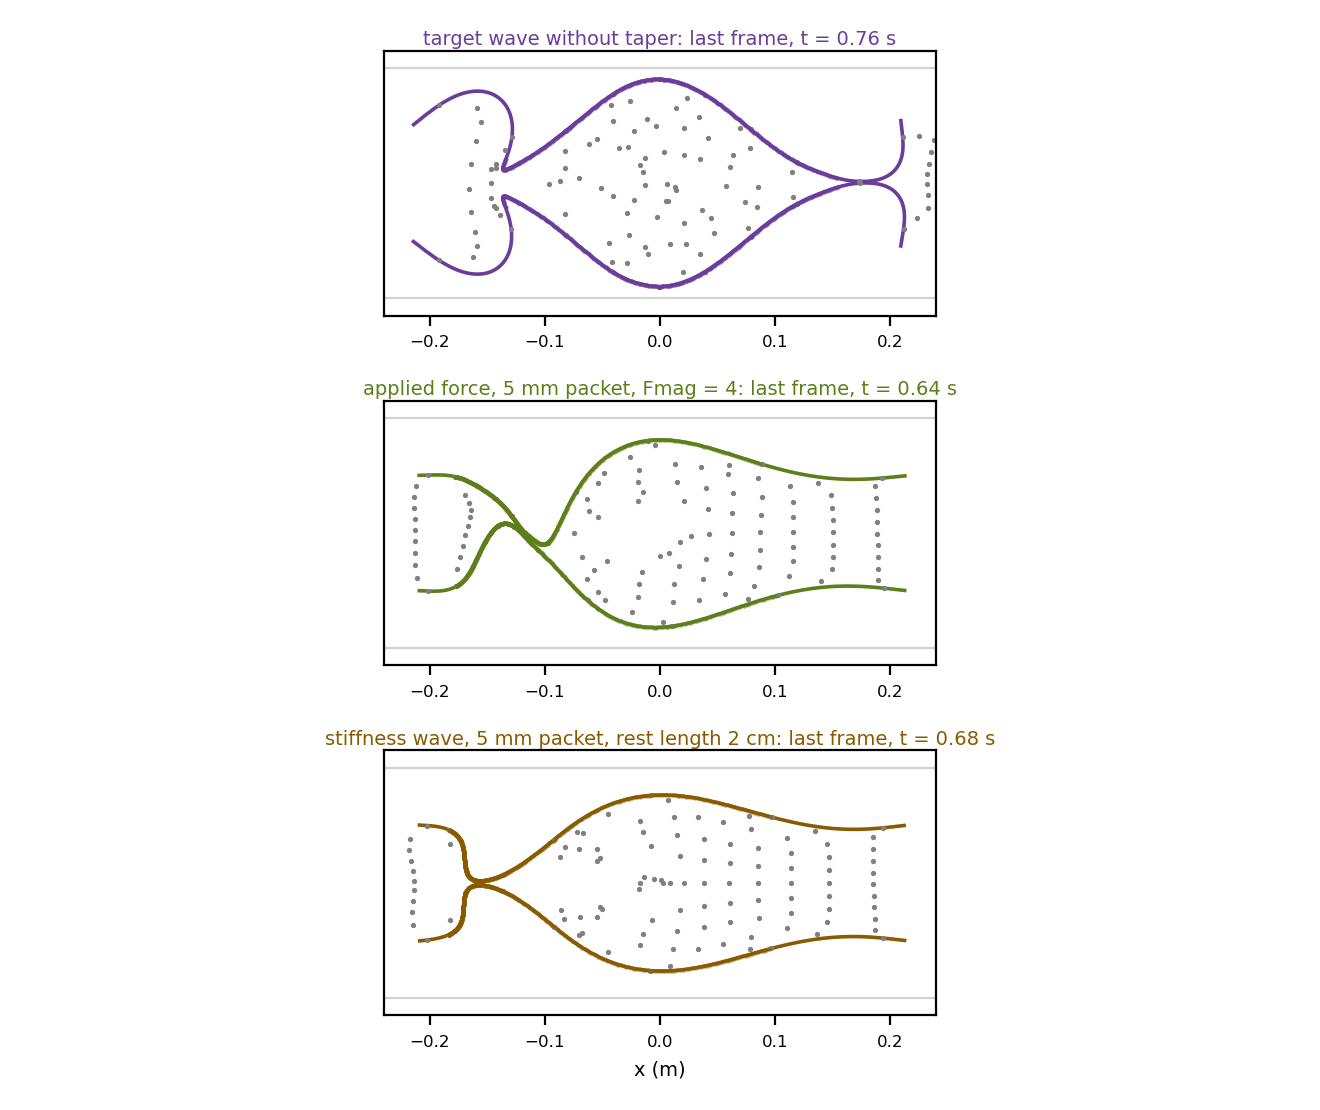
\includegraphics[width=\textwidth]{ch9b-peri-2014}
\end{column}
\begin{column}{0.58\textwidth}
\scriptsize All three stopped between $t = 0.67$ and $0.77$ s with \code{Time step size change encountered} (from the IB integrator's \code{preprocessIntegrateHierarchy}), chapter 16's CFL abort: somewhere the velocity exceeded $0.3\,\Delta x/\Delta t \approx 12$ m/s.
\begin{itemize}
  \item \al{Target wave, no taper} (top): the 2014 wave had a full wavelength on the piece, so its ends moved with it; at $t = 0.75$ s they stood $3.6$ cm proud of the free wall one point away (the folds at $x \approx \pm 0.14$). Fixed by the taper of slide \ref{fr:targetperi}.
  \item \al{Applied force, 5 mm packet, $F_{\mathrm{mag}} = 4$} (middle): the first pinch closed the tube at $t = 0.36$ s and the walls crossed; the pinch never reopened, and the fluid the packet pushed piled up in a bulge that reached the pericardium.
  \item \al{Stiffness wave, 5 mm packet, rest length 2 cm} (bottom): the walls overshot the rest length to $4$ mm apart, two grid cells, and stuck; then as above.
\end{itemize}
\end{column}
\end{columns}
\scriptsize The 2014 code's ad-hoc penalty term was an attempt at the middle case; IB/11 ships a tapered target wave, a wider packet, a gentler force, a longer rest length and, for the applied-force wave, a stiffer tube instead (slides \ref{fr:forceperi}, \ref{fr:kwave}, \ref{fr:fmag}). Tapering the packets themselves was tried and did not help: the collapse is behind the wave, not at the piece's ends.
\sourcecredit{IB/11 with the 2014 update functions and parameters, IBAMR 0.19.0, \code{DT = 5e-5}; last saved frame of each run; \code{tools/ch9b\_figures.py}.}
\end{frame}

% 29
\begin{frame}{Homework}
\label{fr:hw}
\begin{columns}[T,onlytextwidth]
\begin{column}{0.6\textwidth}
\footnotesize From the 2013--2015 courses and this chapter (Appendix C collects the full set):
\begin{enumerate}
  \item IB/11: run \code{TARGET\_VP} and \code{FORCE\_VP}, and find the $F_{\mathrm{mag}}$ at which the applied force gives the same squeeze as the targets. Compare the net flow per period (chapter 29) and the markers' drift.
  \item IB/11: halve $\mathrm{Wo}$ (the viscosity doubles) and halve the frequency, one at a time; say which changes the net flow per period more, which the markers' drift, and why (chapter 8b).
  \item Move the actuator to the middle of the elastic section (\code{Ca} in the generator). What happens to the net flow, and what does that say about valveless pumping?
  \item Write a cable (tension-only) law, register it under index 3, and give it to the springs of IB/01's rubber band. What does the band do when it is compressed?
  \item Write a muscle law with an active tension that the update function raises and lowers at 1 Hz on half of IB/06's fibre.
\end{enumerate}
\end{column}
\begin{column}{0.38\textwidth}
\begin{punchbox}
\scriptsize What to hand in: the force function and its registration line, the generator loop that writes the index, the \code{integral\{F\}} or marker check that shows the force acts, and one VisIt frame per run.
\end{punchbox}
\scriptsize Extension: compute $C_{\mathrm{pump}}$ (slide \ref{fr:cpump}) for the two suction modes from the \code{X.*} and \code{F.*} files.
\end{column}
\end{columns}
\end{frame}

% 30
\begin{frame}{Rules of thumb}
\label{fr:thumb}
\small
\begin{itemize}
  \item A spring function returns the tension from $R$ and the parameters; positive pulls together. No time, no velocity: those come through parameters or a force strategy.
  \item Register under an index other than 0 unless you mean to change every spring; write the index in the fifth column; register before the force generator is handed to the IB method.
  \item Parameters are yours: a force magnitude and a phase are as legal as a stiffness and a rest length. Say what they are in the generator.
  \item Time-dependence: an update function sets a parameter through a reference before each step.
  \item Applied forces can overdo it; a stiffness wave with a rest length cannot; a target wave is kinematics.
  \item The driving structure first in \code{structure\_names}; one input file per mode.
  \item Derivative: exact if you know it, \code{nullptr} if not, never a guess.
  \item Check with \code{integral\{F\}}, the markers, and one frame in VisIt.
\end{itemize}
\end{frame}

% 31
\begin{frame}{Summary}
\label{fr:summary}
\footnotesize
\begin{enumerate}
  \item A spring in IBAMR is a tension law $T(R, \mathrm{params})$ along the line between two points, chosen per spring by an index; the default is Hooke's law, and your own is registered with \code{registerSpringForceFunction(index, \&f, \&df)}.
  \item The 2013 interface (a force vector from a displacement vector and two named parameters) became, in 2015, a tension from $R$ and a parameter array, with an optional derivative; old code ports in a few lines.
  \item Time enters through parameters that an update function sets each step: a phase for an applied force, a stiffness for a travelling wave. The heart-tube pump does this five ways, and the same \code{main.cpp} runs them all.
  \item The applied-force modes trade the certainty of target points for a force the fluid can answer; the stiffness wave bounds the squeeze by its rest length; the pump coefficient measures what each achieves.
  \item For forces that are not between pairs of points there are force strategies, uniform body forces and Eulerian forcing; the two-point pump of chapter 36 needs none of them.
\end{enumerate}
\begin{homebox}
\footnotesize Next, chapter 10: resting curvature and beams, where the preferred curvature of a beam becomes the third kind of prescribed motion.
\end{homebox}
\end{frame}

% 32
\begin{frame}{What changed since the older course notes}
\label{fr:changed}
\footnotesize
\begin{itemize}
  \item The interface is quoted from 0.19.0 and the 2013 one is kept for reading old code; the header's real name is given (\code{IBSpringForceFunctions.h}, not \code{IBSpringFunction.h}) and the default function's (\code{default\_spring\_force}).
  \item The 2014 lecture's code is fixed: the undefined \code{c}, the loop over departed packets, the index-2 registration, the rest-length slot reused as a phase (now documented), and the structure-order dependency (now stated and checked by the mode switch).
  \item The three peristalsis modes were run with the 2014 parameters first and all three aborted at the CFL limit before $0.8$ s (slide \ref{fr:wrong2}); the prescribed wave now tapers at the ends of its piece, the packet's width and speed are input keys, and the shipped values are the ones that run two periods.
  \item The example is assembled from the lab's 2014 \code{Forced-tube-pump} code and the lecture's version of the peristaltic force, with five modes selectable from the input file instead of comments in \code{main.C}; the 2015 public-folder example, which lacked input and structure files, is subsumed. The pumping frequency is read once from the input.
  \item The 2015 slides' ``new addition highlighted in red'' is stated in words, since the highlighting was lost.
  \item New: the zero-derivative explanation, the fifth-column rules from the initializer, the five-mode table, the transport and squeeze figures, the pump coefficient's recipe, the other laws and the other three force mechanisms, the two-point pump preview, and the what-can-go-wrong table.
  \item The 2014 \code{main.C}'s penalty term in the peristaltic force is described but not shipped; the stiffness-wave version it ran is shipped as a mode of its own.
\end{itemize}
\end{frame}

% 34
\begin{frame}{References}
\label{fr:refs}
\scriptsize
\begin{itemize}
  \item IBAMR 0.19.0: \code{include/ibamr/IBSpringForceFunctions.h} (the interface and the default law), \code{include/ibamr/IBStandardForceGen.h} and \code{src/IB/IBStandardForceGen.cpp} (registration, the force loop, the finite-difference derivative), \code{include/ibamr/IBLagrangianForceStrategy.h}, \code{IBLagrangianForceStrategySet.h}, \code{IBMethod.h}; \code{examples/IB/explicit/ex3/example.cpp}. \url{https://github.com/IBAMR/IBAMR}
  \item The example of this series: IB/11 heart-tube pump (\code{main.cpp}, five \code{update\_*.cpp} files, \code{pump\_geometry.h}, \code{generate\_mesh2d.py}/\code{.m}, \code{make\_inputs.py}, five input files, README with the measured results); \code{tools/ch9b\_figures.py}.
  \item The lab's 2014 \code{Forced-tube-pump} code (IBAMR-Examples repository) and the 2014 working folder's \code{notes-gaus-wave} note, the sources of IB/11.
  \item K. Giesbrecht, L. A. Miller and J. Shi, \emph{A theoretical study of two-point dynamic suction pumping} (poster, 2019--2020); the 2019 two-point pump set-up (\code{IBM-SetUp.pptx}, README), the sources of chapter 36.
  \item Sources: \emph{Creating your own spring function in IBAMR} (MATH 769, October 2013); \emph{Designing your own spring force function: examples for peristalsis and dynamic suction pumping} (June 2014, 37 slides); \emph{IBAMR: Creating Spring Force Functions} (A. Hoover, 2015; public folder 14, and 15 ``IBAMR Miscellaneous'').
\end{itemize}
\end{frame}

\end{document}
